% !TEX root = ../team-report.tex
% ERA-Großpraktikum: Team Bericht -- Organisatorisches (Analysis)

\subsubsection{Analyse und Diskussion}
\label{team:orga-plan-anal}

Im Vergleich zwischen dem von uns festgelegten Plan und der Manier, in welcher wir das Projekt tatsächlich bewältigt haben, lassen sich zwei grundlegende Beobachtungen treffen:
\vspace{-0.2cm}
\begin{enumerate}
  \item Aufgrund mehrerer Faktoren ist die Fertigstellung einzelner Meilensteine, vor allem gegen Ende der Arbeitszeit, von obigem Zeitplan merkbar abgewichen,
  \item Dennoch haben wir unsere Vision bis auf wenige Aspekte realisiert und ein vollständiges Produkt entwickeln und abliefern können.
\end{enumerate}

Zusammenfassend kann man sagen, dass wir zwar alle initial festgelegten
Meilensteine erreicht haben, jedoch nicht immer in den geplanten Zeiträumen.
Beispielsweise wurde das Speichermodell nicht wie vorgesehen bereits im Juli,
sondern erst im September fertiggestellt. Ebenso wurde die (korrekte)
Assemblierungslogik zur realitätsnahen Darstellung von Instruktionen im Speicher
im Dezember und nicht bereits im August vollendet. Auch verschob sich ein nicht
unbeachtlicher Teil der Entwicklung der GUI auf Dezember und Januar.
\autoref{fig:commit-history} zeigt ein Histogramm der Commitzahlen auf das
GitHub Repository des Projekts, während \autoref{fig:time-frame} einen Eindruck
über die Diskrepanz zwischen geplanter und tatsächlicher Fertigstellung von
Meilensteinen gibt.

\begin{figure}[b!]
  \centering
  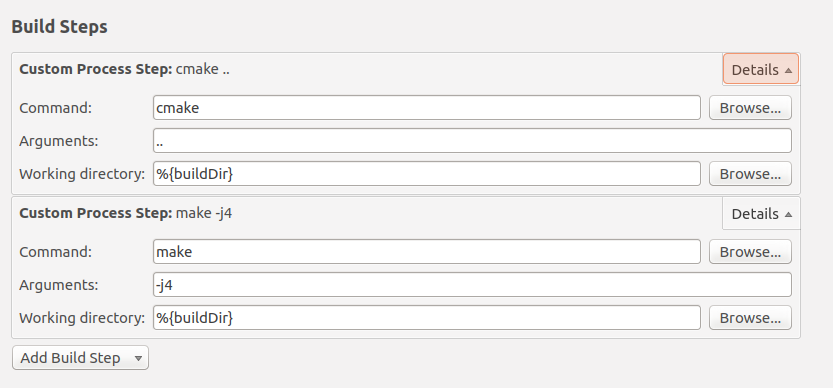
\includegraphics[scale=0.45]{figures/commit-history}
  \caption{Ein Histogramm der gesammelten Commitzahlen auf das GitHub Repository von \erasim{} während des Entwicklungszeitraumes. Quelle: {\small\url{https://github.com/TUM-LRR/era-gp-sim/graphs/contributors}}, letzter Zugriff \today.}
  \label{fig:commit-history}
\end{figure}

\pagebreak
Wir behaupten, dass sich unsere Verplanung bei manchen der Meilensteinen auf drei Ursachen zurückzuführen lässt:

\begin{enumerate}

  \emphitem{Mangel an Erfahrung und Einschätzungsvermögen}. Da zum Zeitpunkt
  unserer Planungsphase kein Mitglied des Teams Erfahrung mit der ``A-Z''
  Entwicklung eines solch anspruchsvollen Projekts hatte, behaupten wir, dass es
  uns schwer fiel, den Arbeitsaufwand für bestimmte Features realistisch
  einzuschätzen. Dies ist insbesondere bei der Entwicklung der GUI merkbar, wo
  gegen Ende der Entwicklungszeit noch viele weitere Hände, als ursprünglich
  geplant, mithelfen mussten, um ein korrektes und intuitives User Interface zu
  gestalten. Könnten wir heute, mit unserer neu gewonnenen Erfahrung, die
  Entwicklungsschritte neu priorisieren, so würden wir bestimmte Aufgaben gewiss
  anders gewichten. \emphitem{Irreguläre Verfügbarkeit}. Während (1) zu Fehlern
  in der \emph{Vorarbeit} geführt hat, war es insbesondere die unregelmäßige
  Verfügbarkeit von Mitgliedern während der Entwicklungsphase, die uns bei der
  \emph{Exekution} der geplanten Schritte Zeit gekostet hat. Bestimmte
  Ereignisse, die im studentischen Alltag auftreten können, seien es
  Prüfungszeiten, Sommerferien oder Praktika, haben es schwer gemacht,
  regelmäßige Sprints zu planen und aufrechtzuerhalten. Beispielsweise erkennt
  man an \autoref{fig:commit-history}, dass gegen Ende Juli und Anfang August
  das Vorbereiten für Klausuren höhere Priorität als die Entwicklung des
  Simulators hatte. Ebenso hinkte im November die Produktivität aufgrund von
  Lern- oder Praktikumsstress sichtlich nach. Diese Unregelmäßigkeit ist
  schlicht ein Resultat davon, dass wir als Studierende an dem Projekt nie
  \emph{vollzeit} arbeiten konnten. Es ist natürlich viel einfacher in einem
  Team von Vollzeitangestellten (bspw. in einer Firma) einen rigorosen
  Entwicklungszyklus einzuplanen und einzuhalten.

  \emphitem{Austritt einiger Mitglieder}. Letztlich identifizieren wir als eine
  weitere Produktivitätsschranke den Austritt zweier Teamkameraden im dritten
  Viertel der Entwicklungszeit. Diesen Mitgliedern waren Aufgaben zugeteilt,
  dessen Abschluss sie uns (verspätet) zusicherten, an welchen sie aber nur
  sporadisch arbeiteten und niemals abschlossen. Als diese Personen dann doch,
  relativ spät, aus dem Projekt vollkommen ausschieden, blieben deren Features
  übrig. Da die bestehende Arbeit dieser Entwickler zum Teil undokumentiert oder
  inkorrekt war, musste noch zusätzliche Arbeitszeit von anderen Teammitgliedern
  investiert werden, um diese Features verspätet aber doch abzuschließen. Im Rückblick hätten wir wohl schneller klarstellen sollen, ob diese Mitglieder sich wirklich weiter für \erasim{} engagieren wollen. Wäre das ``Nein'' als Antwort früher klargeworden, hätten wir deren Aufgaben schneller neu verteilen und fertigstellen können.

\end{enumerate}

\begin{figure}[h!]
  \centering
  \begin{tikzpicture}[thick]
    \draw [|->] (0, 0) -- ++(16, 0);

    \newcount\x\relax
    \x=1\relax
    \foreach \month in {%
      Juni, Juli, August, September, Oktober, November, Dezember, Januar} {
      \draw (\x, 0.125) -- (\x, -0.125) node [below] {\small\month};
      \global\advance\x by 2\relax
    }

    \foreach \name/\planned/\actual/\y in {%
      Speichermodell/3/7/1.6,%
      Assemblierung/5/13/2.4,%
      RISC-V Instruktionen/6/3/3,%
      Direktiven und Makros/5/9/0.8,%
      Ausgabeanzeigen/11/15/3,%
      Verbindung aller Module/3/9/4%
    } {
      \path (\planned, \y) coordinate [fill, circle, inner sep=1.2pt] (p\name);
      \path (\actual, \y) coordinate [fill, circle, inner sep=1.2pt] (a\name);
      \ifnum\actual<\planned
        \newcommand{\arrowcolor}{NavyBlue}
      \else
      \newcommand{\arrowcolor}{Red}
      \fi
      \draw [->, very thick, dotted, \arrowcolor]
            (p\name) -- (a\name) node [above, midway]
            {\color{black}\small\name};
    }

  \end{tikzpicture}
  \caption{Diese Grafik beschreibt die Fertigstellung einer Auswahl an Meilensteinen. Hierbei werden für jeden Meilenstein der geplante und tatsächliche Zeitpunkt der Fertigstellung dargestellt. Pfeile verbinden diese Zeitpunkte, wobei Pfeilspitzen auf das tatsächliche Abschlussdatum zeigen.}
  \label{fig:time-frame}
\end{figure}
